\documentclass[10pt]{beamer}

\usepackage[utf8]{inputenc}
\usepackage{amsmath} % AMS Math Package
\usepackage{amsthm} % Theorem Formatting
\usepackage{amssymb}	% Math symbols such as \mathbb
\usepackage{graphicx} % Allows for eps images
\usepackage{multicol} % Allows for multiple columns
\usepackage{setspace}
\usepackage{fancyhdr}
\usepackage{hyperref}
\hypersetup{
    colorlinks=false,
}
\numberwithin{equation}{section}
\usepackage{verbatim}
\usepackage{siunitx}
\usepackage[font=small,labelfont=bf]{caption}
% \sisetup{scientific-notation = true}
\sisetup{per-mode=symbol}
% \sisetup{output-exponent-marker=\ensuremath{\mathrm{e}}}
\sisetup{load-configurations = abbreviations}

\usepackage{enumitem}
\setitemize{label=\usebeamerfont*{itemize item}%
  \usebeamercolor[fg]{itemize item}
  \usebeamertemplate{itemize item}}
  \usetheme{Hannover}
  \usecolortheme{dove}

\author[Vining]{Melanie Vining}

\institute[UNH]
{
  Integrated Applied Mathematics \\
  Department of Mathematics \& Statistics\\
  University of New Hampshire
}




\logo{\includegraphics[height=1.0cm]{unh_logo.png}}

\AtBeginSection[]
{
\begin{frame}
  \frametitle{Overview}
  \tableofcontents[currentsection]
\end{frame}
}









% \usepackage{beamerthemesplit} // Activate for custom appearance

\title{A Numerically Stable Fourier Continuation Approximation for the Solution of Partial Differential Equations}
\date{\today}

\begin{document}

\frame{\titlepage}

\section[Outline]{}
\frame{\tableofcontents}

\section{Introduction}
\subsection{Motivation}
\frame
{
\frametitle{Motivation}
The Fourier Continuation combined with Alternating Direction (FC-AD) method splits a PDE into a series of one-dimensional BVPs which are then solved using Fourier Continuation approximations.  This research develops and shows new approach to Fourier Continuation approximation that offers greater stability and accuracy.  }
\subsection{FC-AD}
\frame{
\frametitle{FC-AD Overview}
\begin{itemize}
\item Based on Alternating Direction Implicit (ADI) methods
\item Splits the PDE into a series of (the same) BVP 
\item Results in stability as long as the solution to the BVP is stable under that operation
\end{itemize}
}
\frame{\frametitle{FC-AD Computation}
Given the 2-D Heat Equation
\begin{eqnarray}
u_t=k(u_{xx}+u_{yy}) + Q(x,y,t), & (x,y,t) \in \Omega \times (0,T], \nonumber \\
u(x,y,t) = G(x,y,t) & (x,y) \in \partial \Omega, t \in (0,T] \\
u(x,y,0)=u_0(x,y), & (x,y) \in \Omega, \nonumber 
\end{eqnarray}
}
\frame{
\frametitle{FC-AD}
\begin{itemize}
\item Discretize in time, with $t^n = n \Delta t $ and use central difference centered on $t^{n+\frac{1}{2}}=(n+\frac{1}{2})\Delta t$.
\begin{equation}
\begin{aligned}
\dfrac{u^{n+1}-u^n}{\Delta t} &= \dfrac{k}{2}\dfrac{\partial^2}{\partial x^2}(u^{n+1}+u^n) +\dfrac{k}{2}\dfrac{\partial^2}{\partial y^2}(u^{n+1}+u^n)\\& + Q^{n+\frac{1}{2}} + E_1(x,y,\Delta t)
\end{aligned}
\end{equation}
\item Solve for $u^{n+1}$:

\begin{equation}
\begin{aligned}
& \left(1-\dfrac{k\Delta t}{2}\dfrac{\partial ^2 }{\partial x ^2 } - \dfrac{k\Delta t}{2}\dfrac{\partial ^2 }{\partial y ^2 }\right)u^{n+1}\\ &= \left(1+\dfrac{k\Delta t}{2}\dfrac{\partial ^2 }{\partial x ^2 } + \dfrac{k\Delta t}{2}\dfrac{\partial ^2 }{\partial y ^2 }\right)u^n + Q^{n+\frac{1}{2}}+E_1(x,y,\Delta t)
\end{aligned}
\end{equation}
\end{itemize}
}

\frame{
\frametitle{FC-AD}
\small
Expanding and arranging terms gives
\begin{equation}
\begin{aligned}
&\left(1-\dfrac{k\Delta t}{2}\dfrac{\partial ^2}{\partial x^2} \right) \left(1-\dfrac{k\Delta t}{2}\dfrac{\partial ^2}{\partial y^2} \right)u^{n+1}\\ &=  
\left(1+\dfrac{k\Delta t}{2}\dfrac{\partial ^2}{\partial x^2} \right) \left(1+\dfrac{k\Delta t}{2}\dfrac{\partial ^2}{\partial y^2} \right)u^n + \dfrac{k^2 \Delta t^2}{4}\dfrac{\partial ^ 2}{\partial x^2}\dfrac{\partial ^2}{\partial y ^ 2} (u^{n+1}-u^n) \\&+ \Delta t Q^{n + \frac{1}{2}} + \Delta t E_1(x,y,\Delta t)
\end{aligned}
\end{equation}
Here, inverting the operators $\left(1-\dfrac{k\Delta t}{2}\dfrac{\partial ^2}{\partial x^2} \right)$ and $\left(1-\dfrac{k\Delta t}{2}\dfrac{\partial ^2}{\partial y^2} \right)$ gives an expression for $u^{n+1}$ in terms of some $f^{n+1}$.  
}

\frame{
\frametitle{FC-AD}
\normalsize
Inverting the operators on the left hand side results in equations of the form 
\begin{eqnarray}
-\alpha u'' + u= f, & u(x_{\ell})=B_{\ell}, & u(x_r)=B_r 
\end{eqnarray}
}

\subsection{Fourier Continuation}
\frame{
\frametitle{Motivation for using FC}
\begin{itemize}
\scriptsize
\item Fourier Series are known to represent periodic functions well, with cheap computational cost
\item Fourier Series used to represent non-periodic functions experience Gibbs' Phenomenon
\begin{figure}[h!]
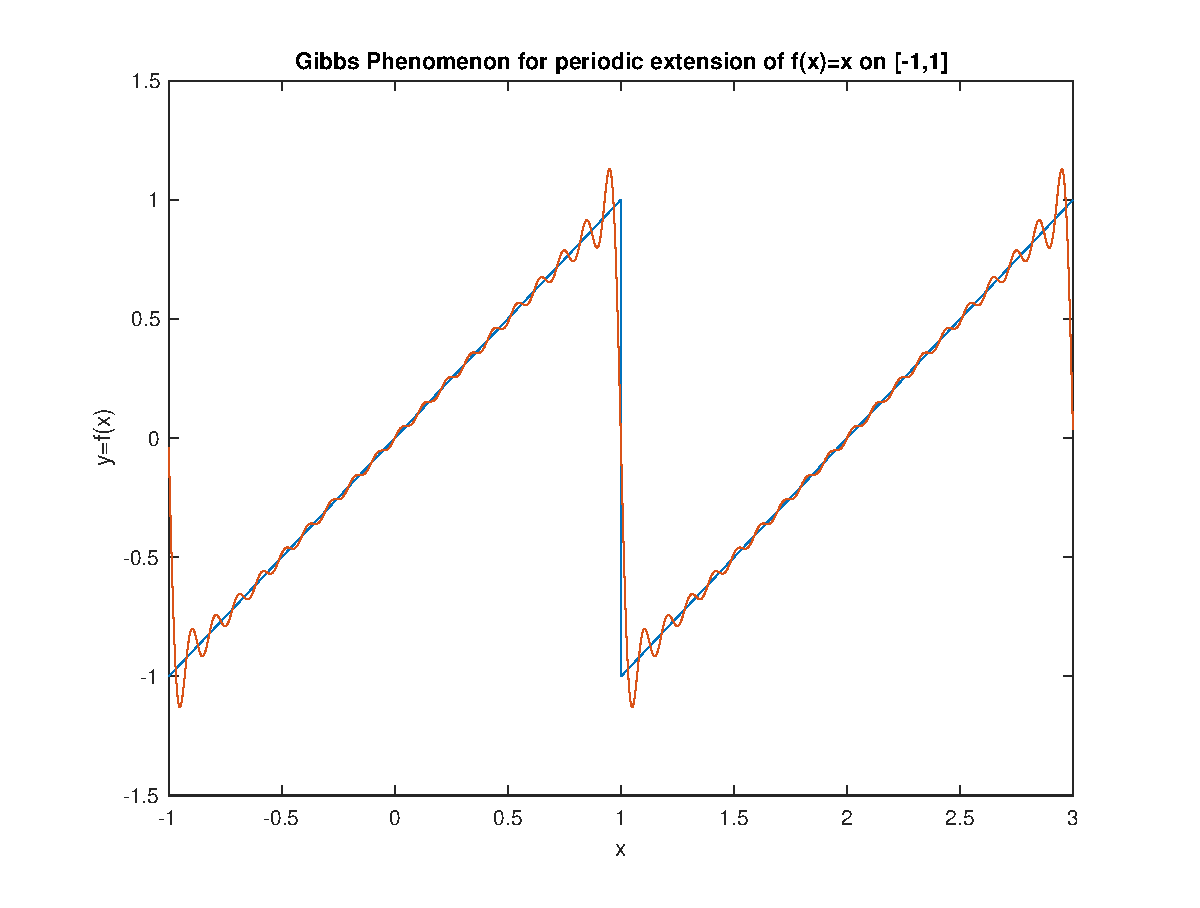
\includegraphics[scale=.25]{Gibbs.eps}
\end{figure}
\item Goal of Fourier Continuation is to get the similar accuracy, convergence, and computational cost with non-periodic functions
\item As a result of using Fourier Continuation approximations, we are given periodic extensions of smooth functions that can be used in conjunction with FFTs to compute numerical solutions to differential equations.
\end{itemize}
}
\frame{
\normalsize
\frametitle{Construction}
\small
Given a smooth function $y=f(x)$ on $[0,1]$ where $f \in C^k[0,1]$, $k>0$.  Discretize the interval onto $N$ points and let $x_j$ be the $j^{\text{th}}$ point on the interval with corresponding function value $y_j=f(x_j)$. 
Choose period $b>1$, and expand in terms of $M$ Fourier Modes, $M<N$, and the problem to solve becomes 
\begin{eqnarray}
y_j=\sum_{k\in t(M)} a_k e^{\dfrac{2\pi i}{b}kx_j}, &j=1\ldots N
\end{eqnarray}
As an example, consider $f(x)=x$ on $[0,1]$.  We discretize on $16$ points, let $b=2$, and $M=7$.  A resulting Fourier Continuation approximation for $f$ is
\begin{figure}[h!]
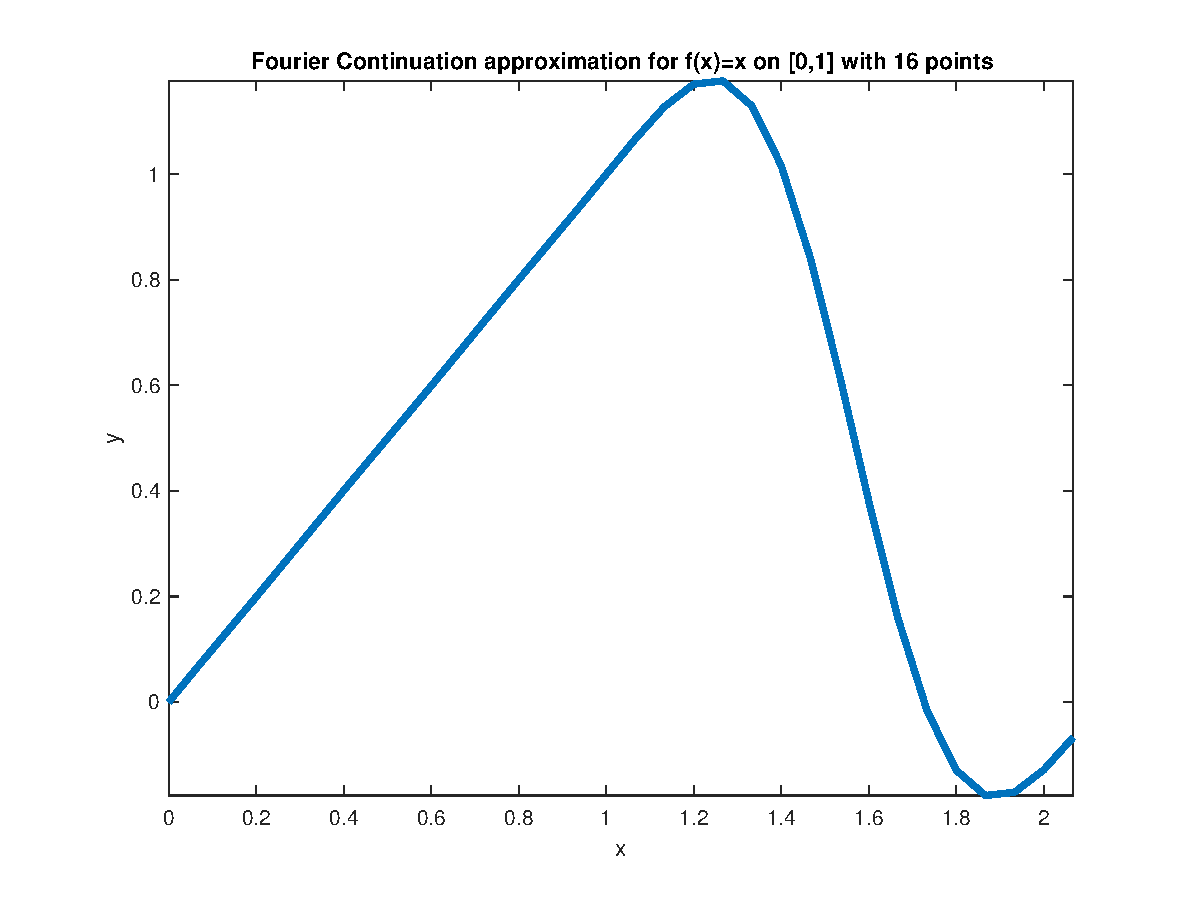
\includegraphics[scale=.25]{FCEx.eps}
\end{figure}
}
\frame{
\frametitle{Fourier Continuation Conclusion}
The previous figure is just \textbf{one} of the possible Fourier Continuation approximations for $f(x)=x$ on $[0,1]$.  Using different methods for solution of the least-squares system can result in different forms. \\
\vspace{.2in}
Is there a ``best" Fourier Continuation approximation for any given problem?

}
\subsection{FC-Gram}
\frame{
\frametitle{FC-Gram}
\begin{itemize}
\item Begin with a basis of polynomials on $n$ points, $f_0,f_1,\ldots,f_{n-1}$
\item Create and store the Fourier Continuation approximations for each of the polynomials
\item Given a function $f$ on any interval with any number of points $m$, sample the first $n$ points and the last $n$ points of $f$.  If $m=n$, use the same $n$ points in order. 
\item Fit the first $n$ points to the basis and the last $n$ points to the basis separately, giving us $a_1$ and $a_2$.  
\item An appropriate combination of $a_1$ and $a_2$ is taken to get a smooth, periodic extension of $f$
\end{itemize}
}

\frame{
\frametitle{FC-Gram Example}
\begin{figure}[h!]
\includegraphics[scale=.5]{FCGram.jpg}
\caption{A comprehensive picture of the FC-Gram method as applied to $f(x)=e^{\sin(5.4\pi x-2.7\pi)-\cos(2\pi x)}$\cite{FCAD1}}
\end{figure}
}
\frame{
\frametitle{FC-Gram Conclusion}
Using FC-Gram to create periodic extensions of functions allows for the use of FFTs and the other ``nice" properties of Fourier Series to be used in solving differential equations.  
}
\section{Current Work}
\frame{\frametitle{Multiple Continuation approximations}
As explained in the Fourier Continuation section, there are several possible Fourier Continuation approximations for the same function.  
\begin{figure}[h!]
\begin{center}
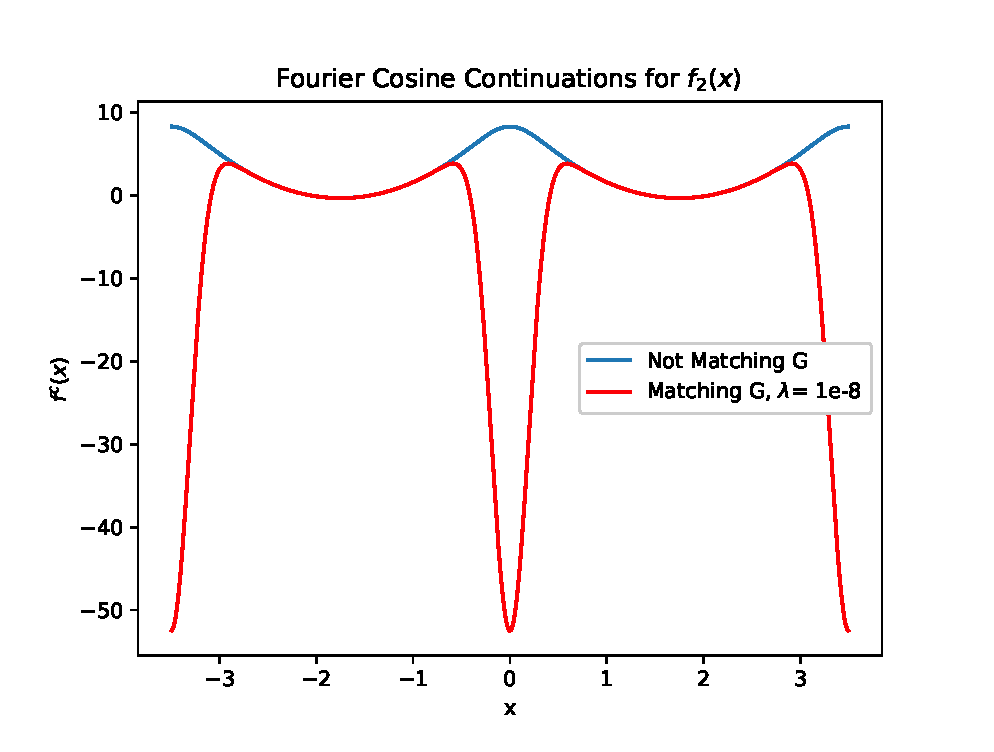
\includegraphics[scale = .3]{f_2ForComparison.eps}
\end{center}
\end{figure}
\normalsize
By adding constraints to the system of equations, we can control the shape of the continuation and ultimately create a stable approximation.  
}
\subsection{Green's Function Solution}
\frame{\frametitle{Green's Function Solutions}
Matching the differential operator to the Green's Function solutions for the given BVP is a natural choice.  The Green's Function solutions are inherently stable under the $\infty$-norm and thus provide the beginning steps for the new form the continuations will take.  
\begin{itemize}
\item Compute the Green's Function for the differential equation $-\alpha u'' + u = f$, $u(x_{\ell})=0$, $u(x_r)=0$. This yields $G(x,a)$.
\item Compute the Green's Function solution as $\displaystyle \int_{x_{\ell}}^{x_r} G(x,a)f(a)da$.  
\end{itemize}
}
\frame{

The calculated Green's Function for $x_{\ell}=-1$, $x_r=b$ is
\tiny
\begin{equation}
G(x,a)=\begin{cases} 
-\dfrac{1}{2} \dfrac{\sqrt{\alpha}\left(-e^{\frac{-1-2b+a}{\sqrt{\alpha}}}+e^{-\frac{a+1}{\sqrt{\alpha}}}\right)\left(-e^{\frac{2(2+b+x)}{\sqrt{\alpha}}}+e^{\frac{2(x+1)}{\sqrt{\alpha}}}+e^{\frac{2(1+b)}{\sqrt{\alpha}}}-1\right)e^{\frac{-x+1+2b}{\sqrt{\alpha}}}}{\left(e^{\frac{2(1+b)}{\sqrt{\alpha}}}-1\right)^2} & x<a \\
\dfrac{1}{2} \dfrac{\sqrt{\alpha} \left(e^{\frac{2+b+a}{\sqrt{\alpha}}} -e^{\frac{a-b}{\sqrt{\alpha}}}\right)\left(e^{\frac{2(-x+b)}{\sqrt{\alpha}}}+e^{\frac{2(1+b)}{\sqrt{\alpha}}}-e^{\frac{2+4b-2x}{\sqrt{\alpha}}}-1\right)e^{\frac{2+b+x}{\sqrt{\alpha}}}}{\left(e^{\frac{2(1+p)}{\sqrt{\alpha}}}-1\right)^2} & x \geq a

\end{cases}
\end{equation}
}
\normalsize
\subsection{Minimization Problem}
\frame{
\begin{itemize}
\item Given $n$ points on an interval, we construct the Gram polynomials $f_0,f_1,\ldots,f_{n-1}$.  Then a sine or cosine continuation matrix is created on a grid, and the functions are evaluated on the same grid. 
\item Next, the function $\tilde{f}$ and its cosine (or sine) continuation $C_u$ are matched, which is the equivalent of solving
\begin{equation}
\min ||C_u f^c - \tilde{f} ||^2 .
\end{equation}
\end{itemize}
}
\frame{
\frametitle{Minimization Problem 2}
\begin{itemize}
\item Using symbolic representations, the Green's function solutions for each of the polynomials are computed and evaluated on the grid. Then a numerical differential operator $I-\alpha\dfrac{\partial^2}{\partial x^2}$ is created for the sine or cosine continuation. 
\item We constrain the original minimization problem using the Green's function and the inverted differential operator applied to the continuation. This yields
\begin{equation}
\min ||C_u f^c - \tilde{f}|| ^2 + ||C_u D_c^{\dagger} f^c - \tilde{G}||^2
\end{equation} 
\end{itemize}
}

\frame{
\frametitle{Minimization Problem 3}
In computation, solving this minimization problem does not achieve great accuracy nor stability.  The homogeneous solutions are not well-represented in the Fourier basis, but the Green's function solution is created from them. An additional constraint is needed in order to allow the system to accurately represent the function while separating out the homogeneous solutions.  Including this constrain modifies the system to
\begin{equation}
\min ||C_u f^c - \tilde{f}|| ^2 + ||C_u D_c^{\dagger} f^c +c_1 \tilde{h_1} + c_2 \tilde{h_2} - \tilde{G}||^2
\end{equation}
where $c_1$ and $c_2$ will be chosen by the computational method to achieve greatest accuracy in the least-squares sense. 
}

\frame{
\frametitle{Minimization Problem 4}
Lastly, two other parameters $\lambda$ and $\mu$ which force the continuations $f^c$ to be stable.  The first, $\lambda$, is applied to control the magnitude of $c_1$ and $c_2$ relative to the homogeneous solutions.  The second, $\mu$ is applied to the coarse-grid point values of the differential operator to control the magnitude of the continuation under the derivative. The final minimization problem we have is
\begin{equation}
\begin{aligned}
\min ||C_u f^c - \tilde{f}|| ^2 + ||C_u D_c^{\dagger} f^c +c_1\tilde{h_1}+c_2\tilde{h_2}- \tilde{G}||^2 \\+ \lambda^2|| c_1 \tilde{h_1} + c_2 \tilde{h_2} ||^2 + \mu^2||C_u D_c^{\dagger}|{\text{\tiny{coarse}}}  ||^2
\end{aligned}
\end{equation}
}
\subsection{Results}
\frame{
\frametitle{Implementation}
We implement this solver in Julia, using 200 bits of precision in \texttt{BigFloat}.  For 200 bits, $\epsilon \approx 10^{-77}$.  With the conditioning of the system, having 77 digits of precision mitigates great error propagation.  The Julia packages \texttt{GenericSVD}, \texttt{SymPy}, and \texttt{PyPlot} were used.  To find the least-squares solution to our minimization problem, we used an SVD and found the pseudoinverse with a tolerance of $10^{-40}$.
}
\frame{
\frametitle{Some Results}
Letting $n=10$, $b=3.5$, setting the unit interval from $1.25$ to $2.25$ and shifting polynomial and Green's Function solution evaluation accordingly, stability was achieved with great accuracy.  Accuracy was computed on a 10 times finer grid, while stability was calculated on the coarse grid of 10 points.  
}
\frame{
\frametitle{Some Results}
Here are two cosine continuations for $f_0$ and $f_1$ with $\alpha = 0.001$:
\begin{figure}[h!]
\centering
\begin{tabular}{|c|c|}
\hline
\includegraphics[scale=.25]{f_0Cosine.eps}

&
\includegraphics[scale=.25]{f_1Cosine.eps}\\
\hline


\end{tabular}
\end{figure}
}
\frame{
\frametitle{Some Results}
Here is a cosine continuation for $f_1$, accompanied by the computed solution $u$, for $\alpha = 0.01$
\begin{figure}[h!]
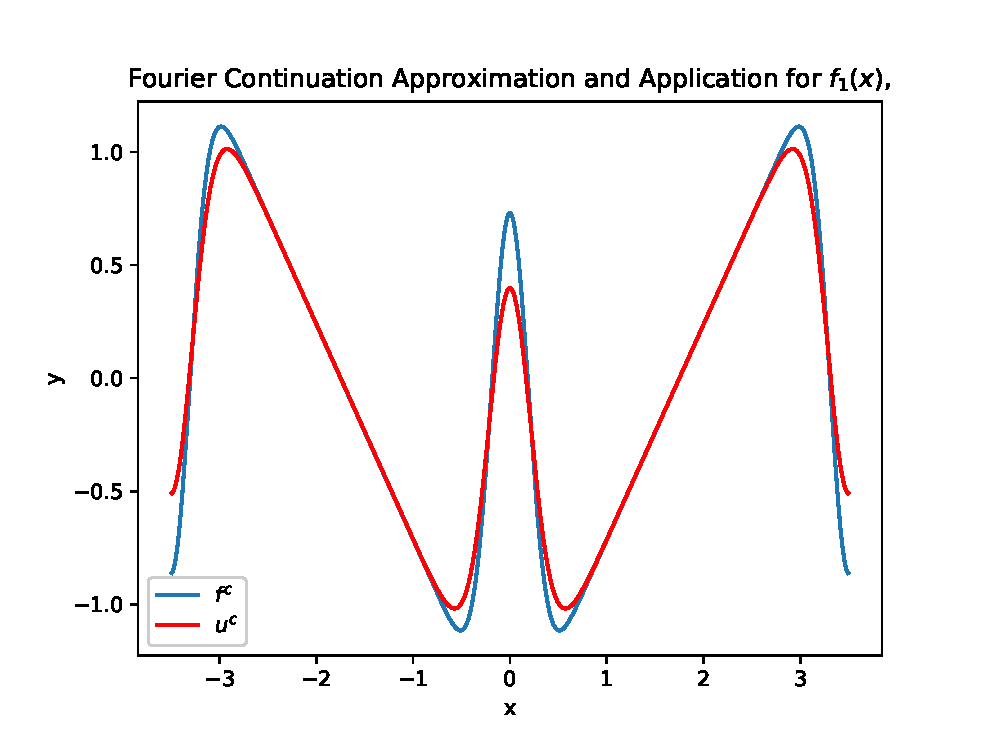
\includegraphics[scale=.45]{f_1u_1.eps}
\end{figure}
}
\frame{
}
\section{Future Work}
\subsection{Computational Work}
\subsection{Analytical Work}
\frame{
\bibliographystyle{unsrt}
\bibliography{citations}
}


\end{document}
